% -*-latex-*-
%
%  The contents of this file are subject to the University of Utah Public
%  License (the "License"); you may not use this file except in compliance
%  with the License.
%
%  Software distributed under the License is distributed on an "AS IS"
%  basis, WITHOUT WARRANTY OF ANY KIND, either express or implied. See the
%  License for the specific language governing rights and limitations under
%  the License.
%
%  The Original Source Code is SCIRun, released March 12, 2001.
%
%  The Original Source Code was developed by the University of Utah.
%  Portions created by UNIVERSITY are Copyright (C) 2001, 1994
%  University of Utah. All Rights Reserved.
%

\section{Concepts}
\label{sec:concepts} 
\index{concepts}

This section describes the general design philosophy and goals of
integrated problem solving environments \index{problem solving
  environment} and how \BIOPSE{} embodies some of these ideas.

\subsection{Traditional Problem Solving Methods}

Traditional methods for solving bioelectric field problems use
multiple, non-integrated computer programs.  For example, using
a computer simulation to examine the effect of electrode patch placement on
transcardiac current density in the design of a cardiac implant-able
defibrillator\cite{CRJ:Sch95b} requires geometric modeling, numerical
simulation, and scientific visualization tools to complete the task.  The
user might need one program to define the thoracic surfaces from medical
images and another to create a discrete mesh of the volume contained within
the surfaces\cite{CRJ:Sch93b}. An application such as Matlab computes a
finite element simulation of the electric current distribution from the
defibrillation electrodes through the thoracic volume\cite{RSM:And93}.
Another approach is to write a Fortran program using a public domain
numerical library such as LAPACK\@ \index{LAPACK}.  To see the output
requires a scientific visualization package (such as those described
in\cite{RSM:All91}).  Between each of these steps, it is necessary to
save the output of one program in a format that the next in the sequence
can read. This process usually necessitates separate file format conversion
utilities.  To find the optimal location, shape, and size parameters for
the defibrillating electrode, the user has to go back to the
geometric modeling package, change the necessary parameters, manually
re-run all of the subsequent steps to see how the new electrode
configuration affects the current density distribution, then manually
iterate.  The manual intervention required to drive this process is
tedious and time consuming.

More efficient is a scenario in which the user can define an
appropriate set of parameters for a given simulation, then set up
a sequence of runs to examine each of them and save the results for
subsequent examinations.  The complete execution of the sequence might
require hours or even days, but the user is free during that
time to perform other tasks.  This process is similar to the ``what
if?'' analysis that modern spreadsheet programs offer for far simpler
problems.  

In the example of the defibrillation simulation, the user can
select various locations and orientations for the defibrillation
electrodes, choose values for other parameters of the simulation
(\eg{} the number of nodes in the finite element model, the boundary
conditions, the error tolerance for convergence, and the evaluation
criteria), and leave the simulations to run as long as necessary.
Viewing the results can be as simple as watching the animation
produced by the simulation or scanning other defibrillation quality
indices such as maximum and minimum current density magnitude or
current density histograms from the heart.  This automated execution
process, whereby the user selects all of the parameters in advance and
does not control the intra- or inter-package execution is called
\emph{batch processing}.  A benefit of batch processing is
that it allows the user to utilize computational resources
without intervention.  However, most scientific computer software
 requires some user intervention in order to
produce meaningful results .  This constraint makes it difficult or
impossible to run multiple computational jobs automatically, leaving
the user with the task of manually initiating and controlling each
step of the process.

\subsection{Integrated Problem Solving and Computational Steering} 
\label{sec:con-steering} 

The goal of integrated problem solving environments, specifically
of \SR{} and \BIOPSE{}, is to integrate the steps
described in the previous example as components in a single, unified,
extensible problem solving environment \index{PSE}.  The resulting function
includes the ability to manage each step in a
sequential computing process, and to create batch processes that
execute repeated simulations. The functionality that sets
\SR{} and \BIOPSE{} apart from most integrated software environments
is the ability to intervene and control execution anywhere in the
chain at any time during its execution.  The ability to control a
computer program during execution is termed \emph{computational
  steering.}

To provide a non-technical analogy, adding computational steering to a
software environment is similar to adding the ability to 
switch tracks in train travel.  A train passenger can get on a train
and get to a new destination, leaving all the details of
the individual actions to the rail system machinery and staff. The route and the 
destination are fixed.  Steering would permit each
passenger, at any time during the trip,  to request that the train take a new route, with different
stops, and a different destination.  In the example
of the defibrillation simulation, computational steering allows users to interactively change parameters and settings as the
simulation executes, performing his or her work in batch and interactive
modes.  Steering interventions might include adjusting electrode
locations to stay within anatomically reasonable bounds or refining
the geometric model resolution in order to balance accuracy and
execution time.

To achieve integration within the elements of \SR{} and \BIOPSE{},
data flows directly from one processing step to the next, without
being diverted to a disk file or leaving the program.  Output from
each step is available as input to dependent steps.  The underlying
paradigm of \SR{} is data flowing between modules that each perform
some operation.  Integration between modules guarantees that upon
completion of their tasks, upstream modules pass their data to
downstream modules, thereby forcing the downstream modules to execute
in response.  In the computational steering example,  the user may alter
electrode locations at any time, initiating a sequence of all
necessary steps to recompute the simulation with the new
configuration.  The modification of the geometric model, finite
element calculation, and visualization all proceed automatically and
in the proper sequence, all managed by \SR{}.  The combination of
steering and component integration allows the user to
spontaneously explore a problem.

While computational steering is a young field in computer
science, there are a number of examples of such systems (in addition
to \SR{}) described in the literature.  Burnett\cite{MM:Bur94}, and
Vetter and Schwan\cite{MM:Vet96} give overviews of existing
computational steering systems. Notable examples include
CUMULVS\cite{MM:Gei96,MM:Koh97}, \index{CUMULVS}
Progress\cite{MM:Vet95}, \index{Progress} and Magellan\cite{MM:Vet97a}
\index{Magellan}.



\subsubsection{\SR{} and its Packages}
\label{sec:srversuspse}

%begin{latexonly}
\newcommand{\eabfig}{%
  \includegraphics{../FAQ/EAB-BioPSE.eps}
}
%end{latexonly}
\begin{htmlonly}
  \newcommand{\eabfig}{%
    \htmladdimg[align=left,alt=""]{../../FAQ/EAB-BioPSE.gif}
  }
\end{htmlonly}

It is important to understand the place of the software included in
this package within the hierarchy of computational problem solving
environments developed at the SCI Institute.  From a historical
perspective, \SR{}, which began development in 1992, was the
original implementation of the computational
framework\cite{CRJ:Joh94c,RSM:Par95,RSM:Par95b,RSM:Par97,RSM:Par97b,CRJ:Parker99b}.
Since then, \SR{} and its computational workbench infrastructure has
been the basis of many significant application-specific projects. 
Examples are the DOE sponsored Uintah system \cite{RSM:Dav2000}
and the NIH sponsored \BIOPSE{} system.  The target applications of
the Uintah project are combustion, computational fluid dynamics, and
mechanical modeling implemented on large-scale, distributed, shared
memory architectures.  The goal of the \BIOPSE{} project is to create
software for geometric modeling, simulation, and visualization for
solving bioelectric field problems.  A secondary goal of
the \SR{} system is to make source code for  problem solving
environments available to the scientific community.

\begin{figure}[htb]
  \centering
  \begin{makeimage} \end{makeimage}
  \eabfig
  \caption{\label{fig:eab-BioPSE} \sr{} and its
    packages.  BioPSE, for example, consists of \sr{}
    the BioPSE package.}
\end{figure}

To support extensibility in \sr{}, its infrastructure has undergone
significant reorganization, extension, and enhancement. \SR{} remains
the core problem solving environment and the name is used to refer to
the entire ensemble of software.  A user may now use the core \SR{}
software and augment its functionality with one or more packages such
as \BIOPSE{} (as shown in Figure~\ref{fig:eab-BioPSE}).  \sci{}
anticipates the collection of packages will grow as the \SR{}
infrastructure becomes available to scientists and engineers in varied
disciplines.

In addition to major projects that have leveraged and
advanced \SR{}, there exist a number of smaller packages that extend
\SR{}'s utility.  Examples include the Teem package for raster data
processing, the NetSolve package for linear algebra subroutines
(developed by researchers at the University of Tennessee and
Knoxville), and a communications interface to the Matlab program.  \SCI{}
has developed various forms of software wrappers or interfaces that
allow \SR{} to leverage the strengths of these third party tools,
links referred to as "bridges."

There are instances when a tighter level of integration than a
bridge between \SR{} and third-party software is necessary.  One example
is the addition of MPEG support for capturing animations from the \SR{}
Viewer module, for which the Berkeley and Alex Knowles' MPEG
encoding tools are used.  Another example is the set of image generation and
manipulation tools from Peter Haeberli called libimage.  To indicate
whether or not such tools are available, the configure scripts for \SR{}
contain optional control flags.

\sci{} believes the combination of a robust infrastructure and modular
extensibility through packages and third-party libraries will allow \SR{}
to grow, and adapt to changing needs and opportunities. 

This manual will be consistent with the usage of the
terms \SR{} and \BIOPSE{}.  \sr{} will typically refer to some feature that
is common to the core functionality of the system. This is common to all
of the problem solving environment application packages.  \BIOPSE{} will
refer to specific elements of the bioelectric field problem solving
environment.


\subsection{\SR{} Modules and Networks}
\label{sec:con-modules} 

%begin{latexonly}
  \newcommand{\basicmodule}%
  {\centerline{
\epsfig{file=Figures/biopse-modmap.eps.gz,width=\columnwidth,
  bbllx=7, bblly=-193, bburx=774, bbury=14}}}
%end{latexonly}
\begin{htmlonly}
  \newcommand{\basicmodule}{%
  \htmladdimg[align=top,width=766,alt="module"]
  {../Figures/biopse-modmap.gif}}
\end{htmlonly}

The functional unit of a dataflow environment is the {\em\/module}
\index{module}.  Figure~\ref{fig:conc-module} contains a generic \SR{}
module, with a User Interface (UI) button for graphically accessing the
module's user interface, and input and output ports for receiving and sending
data, respectively.  On the right is a simple example of a dataflow
network.  Data passes through the output port of the top module, through
the data pipe, and into the input port of the bottom module.  The User
Interface enables the selection of a desired isochrone surface.

\begin{figure}[htb]
  \begin{makeimage}
  \end{makeimage}
  \basicmodule
%  \centerline{
\epsfig{file=Figures/biopse-modmap.eps,width=6in}}
  \caption{\label{fig:conc-module} Example of a \SR{} module}
\end{figure}

Modules may contain other elements, but all have at least one input or
one output port. Most modules have input and output ports connected to
other modules.  Data readers are modules with only an output port.
Their ``input'' is read from a file.  The
\htmladdnormallink{\emph{Viewer}}{viewer.html} module provides input
ports only; scene data arrives on its input ports and a screen
visualization is its ``output''.  

It is important to appreciate the concepts of modules, connections
between modules, and the dataflow through a network (see
\secref{Working with Networks}{sec:workwithnets} for more information
on modules, ports, connections, and networks).


\subsection{\sr{}'s Use of Third Party Software}
\label{sec:con-links} 

\SR{} works with software from third party sources in several
ways. The use of third party software is largely invisible to the user of \SR{} or
\BIOPSE{}.

For example, \sr{}'s user interface is written in the Tcl language
using the Tk library.  In general, \sr{}'s modules use Tcl for their
user interface elements and C++ for their computations.  However, a
module may also interact with code written in other languages such as
FORTRAN or Matlab.

One goal of the \BIOPSE{} project is to provide
support for such external code, including FORTRAN, C, Matlab, and
IDL\@.

\subsubsection{Matlab}
\label{sec:concept-matlab} 

The interface (based on Berkeley sockets) between \SR{} and Matlab provides
a pathway to send matrix data objects from \SR{} to Matlab, then accepts
the results of some Matlab computations.  Currently, this arrangement
requires a Matlab script to perform the desired
operations.  \SR{} sends the input data to an existing process running
Matlab, which serves as a compute engine. Matlab then performs the steps
described in the script, and returns data to \SR{} for further
processing or display.  The Matlab process can run on a separate
computer connected via a network, helping to distribute the load and resolving potential licensing conflicts with Matlab.

The underlying mechanism for this communication is a socket interface
consisting of two \SR{} Modules, \module{MatrixSend} and
\module{MatrixReceive}, and a Matlab ``transport'' routine. The \SR{}
and the Matlab processes know each other's whereabouts (in the form
hostname:port) and use a client-to-client communication model.
Synchronization between processes is manual.  For example, 
the \SR{} \module{MatrixSend} module sends the matrix to a socket where a 
Matlab script is listening.  The script receives the matrix, 
performs the calculations in Matlab and sends the results to a socket 
where \module{MatrixReceive} module is listening.  \SR   then carries out
further calculations and displays the results.

%For examples of this interface, see \secref{Matlab
%Examples}{sec:examples-matlab}.

\subsubsection{GENESIS (via SQL)}

\htmladdnormallink{GENESIS}{http://www.bbb.caltech.edu/GENESIS/genesis.html}
(short for GEneral NEural SImulation System) is a general purpose
simulation platform which was developed to support the simulation of neural
systems ranging from complex models of single neurons to simulations of
large networks made up of more abstract neuronal components. GENESIS has
provided the basis for laboratory courses in neural simulation at
Caltech and the Marine Biological Laboratory in Woods Hole, MA, as well as
many other institutions.   

\sci{} has created a bridge between \SR{} and GENESIS so it is possible
to use the output of a GENESIS simulation as the input for a
visualization, or a subsequent simulation within \BIOPSE{}.  The mechanism for
this bridge is a database accessible via SQL queries.  \sci{} created
code for GENESIS that writes the output of the simulation into the database, then the corresponding functions for \SR{} read this
information from the same database.   Contact Chris Butson
\htmladdnormallink{butson@sci.utah.edu}{mailto:butson@sci.utah.edu}
for details about the implementation of the GENESIS module.


\subsubsection{PETSc}

\htmladdnormallinkfoot{The Portable, Extensible, Toolkit for
  Scientific Computation
  (PETSc)}{http://www-unix.mcs.anl.gov/petsc/petsc-2/} is a library of
data structures and functions for the parallel solution of partial
differential equations.

When PETSc is installed (and SCIRun is configured to use it), SCIRun's
\module{SolveMatrix} module enables the use of PETSc solvers.

Installation of PETSc is optional. SolveMatrix provides built-in
solvers if PETSc is not available.

\subsection{Extensibility}
\label{sec:con-extend} 

\SR{} is an extensible \index{extensible} problem solving environment.
This is true in the sense that there are no limits to the
different ways of connecting modules and creating new applications.  

\sr{} can also be extended by creating new packages and modules.
Modules can be coded from scratch or with the assistance of the
\sr's \dfn{Module Maker} component.

\sci{} anticipates users  creating new modules. \sci{} 
encourages users to contribute modules to a repository on the \BIOPSE{}
web site \index{BioPSE@\BIOPSE{}!web site} 
(\htmladdnormallink{www.sci.utah.edu/ncrr/software/biopse.html} 
{http://www.sci.utah.edu/ncrr/software/biopse.html} where they will be reviewed, and useful modules will be included in subsequent releases of \sr{}.
Future releases will include more extensive tools for building modules
and wrapping existing codes within \SR{} module wrappers, to maximize
intellectual investment in legacy code.

\subsection{\sr{} Objects}
\label{sec:sr-objects}


\sr{}'s \datatype{Field}, \datatype{Mesh}, \datatype{Matrix}, and
\datatype{ColorMap} objects are used frequently in networks.  These
objects are described in sections that follow.

\subsubsection{Field}

A \sr{} \datatype{Field} consists of a geometric \datatype{Mesh} and a
set of data values.  Data values can be located at the nodes, edges,
faces, or cells of a mesh.  A \datatype{Field} can consist of a
\datatype{Mesh} component only (no associated data).

\subsubsection{Field Data}

The following C++/SCI data types can be associated with a \datatype{Field}:

\begin{itemize}
\item \datatype{double}, \datatype{float}
\item \datatype{int}, \datatype{short}, \datatype{unsigned}, \datatype{unsigned short}
\item \datatype{char}, \datatype{unsigned char}
\item \datatype{Tensor}
\item \datatype{Vector}
\end{itemize}

C++ data types are \datatype{double}, \datatype{float},
\datatype{int}, \datatype{short}, \datatype{unsigned},
\datatype{unsigned short}, \datatype{char}, and \datatype{unsigned
  char}.  \sr{} data types are \datatype{Tensor} and \datatype{Vector}.

\subsubsection{Meshes}

\sr{} meshes are classified as \dfn{unstructured}, \dfn{structured}, or
\dfn{regular}.  In general, a mesh consists of nodes (data value location
data) and node connectivity data.

Node locations and connectivities for unstructured meshs are specified
explicitly.  The unstructured mesh types are:
\datatype{PointCloudMesh}, \datatype{CurveMesh},
\datatype{TriSurfMesh}, \datatype{QuadSurfMesh},
\datatype{TetVolMesh}, \datatype{HexVolMesh}.

Node locations are specified explicitly and connectivities are known
implicitly for structured meshes.  The structured meshes are
\datatype{StructCurveMesh}, \datatype{StructQuadSurfMesh}, and
\datatype{StructHexVolMesh}.

Node locations and connectivities are known implicitly for regular
meshes.  The regular mesh types are \datatype{ScanlineMesh},
\datatype{ImageMesh}, \datatype{LatVolMesh}.

Below are figures of some mesh types:

%begin{latexonly}
\newcommand{\meshdoc}[4]{%
  \includegraphics[0,0][100,#1]{Figures/#2.eps.gz}
  {#4}
}
%end{latexonly}
\begin{htmlonly}
  \newcommand{\meshdoc}[4]{%
    \htmladdimg[align=left,alt="#3"]
    {../../Tutorial/images/figures/#2.gif}
    #4 \begin{rawhtml}<br clear="all"/>\end{rawhtml}
  }
\end{htmlonly}

\meshdoc{100}{pointcloud}{Point Cloud Mesh}{A Point Cloud mesh is a
  set of unconnected points.}

\meshdoc{60}{ScanlineField}{Scanline Mesh}{A Scanline Mesh is a
  regularly segmented straight line (a regular 1D grid).}

\meshdoc{60}{ContourField}{Contour Field Mesh}{A Curve mesh is a 
  segmented curve.}

\meshdoc{100}{ImageField}{Image Mesh}{An Image mesh is a regular 2D
  grid. Note that an Image mesh is not used for image processing because
  \sr{} does not support that function.}

\meshdoc{65}{trisurf}{Tri Surface Mesh}{A Tri Surface mesh is a
  surface made of connected triangles.}

\meshdoc{83}{quadsurf}{Quad Surface Mesh}{A Quad Surface mesh is a surface made of connected quadrilaterals.}

\meshdoc{87}{latticevol}{Lat Vol Mesh}{A Lattice Volume mesh is a regular 3D grid.}

\meshdoc{60}{tetvol}{Tet Vol Mesh}{A Tet Volume mesh is a subdivision of space into tetrahedral elements.}

\meshdoc{84}{hexvol}{Hex Vol Mesh}{A Hex Volume mesh is a subdivision of space into hexagonal elements.}


\subsubsection{Matrices}

\sr{} supports three matrix types: 

\begin{description}
\descitem{\datatype{ColumnMatrix}} An \(Mx1\) matrix using \(M\)
storage units.

\descitem{\datatype{DenseMatrix}} An \(MxN\) matrix using \(MxN\)
storage units.

\descitem{\datatype{SparseRowMatrix}} A \(MxN\) matrix where most
elements are zero and no storage is allocated for zero valued
elements.
\end{description}

\datatype{ColumnMatrix},
\datatype{DenseMatrix}, and \datatype{SparseRowMatrix}.

\subsubsection{Color Map}

\sr{} \datatype{ColorMap} type is a mapping of color values to data values.

%%% Local Variables: 
%%% mode: latex
%%% TeX-master: "usersguide"
%%% End: 
